\documentclass{tufte-book}

\usepackage{graphicx}
\setkeys{Gin}{width=\linewidth,totalheight=\textheight,keepaspectratio}
\graphicspath{{graphics/}}

\usepackage{xcolor}

\usepackage{listings}
\lstset{
	basicstyle=\ttfamily\small,
	breaklines=true,
	breakatwhitespace=true,
	xleftmargin = 0cm,
	xrightmargin = 0cm,
	framexleftmargin = 0.2em,
	frame=tb,
	literate={~} {$\sim$}{1}	% to make tilde be centered vertically
}

\usepackage{geometry}

\geometry{
	% showframe,
	paperwidth=8.5in,
	paperheight=11in,
	left=0.71in,
	%right=0.45in,
	top=0.61in,
	%bottom=.5in,
	textwidth=4.96in,
	marginparsep=0.35in,
	marginparwidth=1.77in,
	includehead,
	% The text width and height are calculated automatically.
}

\usepackage{url}

\title{Delve into ESP32}
\author{Henrik Samuelsson}

\begin{document}
\maketitle

\cleardoublepage
\chapter*{Development Tools Setup}

This chapter discusses hardware and software needed to have to be able to do the exercises and projects presented in this book. The best way to learn is by experimenting and trying real things by yourself as opposed to just reading theoretical background material or watching videos.

A number of different components are required to complete all the projects presented in this book. If your budget is limited so will you be  able to do many of the projects with just a handful of components, and each one is not really expensive either.

\section{Mandatory Hardware}\label{sec:hardware}
The following things is a must if you really want to become familiar with the ESP32.

\begin{itemize}
	\item Computer for development of software to be run on a ESP32
	\item ESP32 development kit
	\item Bread board
	\item A basic selection of passive and active electronic components
\end{itemize}

Each type of needed item is discussed more in detail in the following sections.

\subsection{Development Computer}
A computer running Linux, Windows or macOS is needed to build the software to be run on the ESP32. The bulk of the projects in this book have been developed and tested on a computer running Ubuntu 16.04, so this is the preferred operating system. Everything should, at least in theory, work under other operating system but the ride might not be as smooth.

Hardware specs on the computer are really not high. Computer to be used should have one or two free USB ports. There must also be some free disk space for software development tools. Other than that so should pretty much anything work.

\subsection{ESP32 Development Kit}
A development board with an ESP32-WROOM module is considered mandatory to be able to test the programs that you will create. Espressif, the company behind the ESP32, have released a development board named ESP32-DevKitC that can be bought for about \$15. Do a web search and you should find several vendors that sell it on for example eBay or Amazon. It could also be so that your own favorite electronic components vendor have it in stock.

There are also various variants of the official development board developed by third parties. The cheapest ones can primarily be found on Chinese on-line market places. This can be a way to save a little money but there will usually be a few weeks of waiting for the order to arrive if you do not live China.
frame=tb,
An USB cable is needed to connect the development board and your computer. Exact cable needed depends on the computer and what development board being used. USB A to micro USB is probably the type that you need. Check the ports of your computer and the connector on the development kit before buying.

\subsection{Bread Board}
Many of the projects requires various electronic components to be connected together. A fast way to hook up components is by using so called bread boards. Bread board comes in various colors and sizes see below picture for an example of a board with 830 connection points.

\begin{figure}
	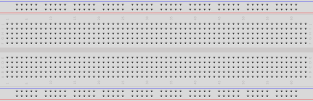
\includegraphics{bread_board.png}
	\caption[Bread board $n$.][6pt]{A common type of bread board. There are plenty of connections points and rails for dual supply voltage.}
	\label{fig:bread_board}
\end{figure}

The ESP32-DevKitC is bread board friendly and can be plugged in to the bread board directly. But it is fairly wide and will cover many connection points that we will want to have free to be able to connect other things. The solution is to have multiple boards connected together by the same principle used as when laying a jigsaw puzzle. Notice the three small knobs on the bottom of the board in the picture these will fit holes located at backside of the the top of the board. The board you want to have should be of this type that can be connected together with other boards. So search for a ''830 bread board`` that is specified to be able to be connected together and buy two off these boards. 

An alternative is to search for ''1660 bread board`` and you will get hits were two bread boards are already mounted together for you on a metal plate.

Choose either one of these two options but make sure that the bread boards have gotten good reviews by other users because there are a lot of products out there that works less well. 

\subsection{Electronic Components}
A basic supply of electronic components will be needed for the projects. The components can be bought as separate units but it is easier and usually cheaper to buy a complete kit. There are starter kits, sufficient for our needs, that can be bought for around \$15. These kits can be found at the same places where you buy your ESP32 development kit. Search for ``Arduino starter kit'' or ``bread board starter kit''. Note that the the kit does not need to contain an actual Arduino micro controller, the ESP32 will play the role as the controller in our projects.

The following list summarizes some of the components that should be included in your collection of electronic components.

\begin{itemize}
	\item Jumper wires
	\item Dupont wires
	\item An assortment of different resistors
	\item Some different ceramic and electrolytic capacitors
	\item Push buttons
	\item LED's in some different colors 
	\item Potentiometer
\end{itemize}

\section{Software}\label{sec:software}

The process of getting the ESP32 to run our own software depends on the steps and building blocks illustrated in figure~\ref{fig:software_anatomy}.

The very basic foundation of our software will be some packages that we must have on our development computer. On top op these packages so is there a library of ESP32 specific code provided by Espressif. This library is called Espressif Internet of Things Development Framework (ESP-IDF). This library abstracts away some of the hardware specific details and speeds up the development. The final piece of code that can be seen in figure~\ref{fig:software_anatomy} is labeled Our code and this will be project specific code written by us to make the ESP32 do what we want it to do.

When we are done writing a part of our code and shall test it so will we first build a binary file, this is done by running programs and scripts from a set of tools refereed to as the tool chain. A binary file will be the result of an successful build. This binary shall finally be download to a ESP32 and if we have written to code correctly so will the ESP32 start executing the code and start to behave as we intended. 

\begin{figure}
	
\includegraphics[scale=1.0]{software_anatomy.png}
	\caption[Software development $n$.][6pt]{Overview of the software blocks and steps needed to get an application running on the ESP32.}
	\label{fig:software_anatomy}
\end{figure}

\subsection{Software Installation}
Exact way to install the software needed to be able to build for the ESP32 depends on what operating system your development computer is running.
Only installation instructions for Ubuntu Linux is provided in this book as an illustrative example. Instructions for all supported operating systems including Ubuntu Linux can be found by searching on-line for ''Espressif ESP32 installations instructions``.
Even if you choose to follow the software installations instructions that can be found on-line so is it a good idea to glance through the instructions in the sections that now follow since there are, aside from the Ubuntu specific instructions, some general useful information that is valid for all installations regardless of the underlying operating system.

\subsection{General Software Packages Installation on Ubuntu Linux}
There are, as already discussed, a number of software packages that are needed to be able to program an ESP32. Make sure that all of these are available by opening a terminal window and execute the following command. 

\marginnote{There shall not be any line breaks in the command that you type in. The line break and tab in the command are just present for layout reasons to be able to fit the command on the page of this book.}
	
\begin{lstlisting}
sudo apt-get install git wget make flex bison libncurses5-dev gperf python python-serial
\end{lstlisting}

Expected result is that the apt-get utility, a package management command line program that handles Ubuntu's Advanced Packaging Tool library, should perform installation of some new software packages.
 
Check the resulting output in the terminal for eventual problems occurring during the installation process. Should one or more packages fail to install so should you try to fix this before continuing with the next installation steps. Not having all the packages will most likely cause problems later on. Search for information on-line or post a question at the ESP32 forum that is located at www.esp32.com to resolve eventual issues.

\subsection{ESP-IDF Retrieval}

\marginnote{GitHub is a web-based Git or version control repository . It is mostly used for code. It offers all of the distributed version control and source cThe purpose of the tool chain is to combine the source code that we write with source code from others such as for example code fromode management functionality of Git as well as adding its own features.}

The official development framework for the ESP32 is called ESP-IDF. More or less all projects in this book will use functionality from this framework. ESP-IDF can be retrieved from GitHub and it will now be explained how to download a clone of the framework to your development computer.

Open a terminal and move to a location where you want to store the code to be downloaded. It is assumed that you will create a folder named esp that will hold various sub folders for the purpose of storing ESP-IDF files. This esp folder will also later on be the parent folder for the tool chain and example project as well as your own projects for the ESP32.

\marginnote{The ESP-IDF is under active development and it could be so that there is a later release available by the time you are reading this. You can choose to get this later release instead of version 2.1. Benefits of this would be to get bug fixes and extended functionality. The down side to choosing a later release is that it may not be one-hundred percent backwards-compatible so it could break some of the code presented in this book.}

The latest current release, at the time of writing, is version 2.1. To get this release, use the following commands in a terminal.

\begin{lstlisting}
git clone https://github.com/espressif/esp-idf.git esp-idf-v2.1
cd esp-idf-v2.1/
git checkout v2.1
git submodule update --init --recursive
\end{lstlisting}

Expected result from these commands are the following. A new folder called esp-idf-v2.1 is created on your computer. This folder should hold various documents and folders such as for example components, docs, examples, make. The checkout command and the submodule update command ensures that the version of the ESP-IDF framework is in the same exact state as it was when release 2.1 was made.
You should now stop reading and instead write down a note of the version of ESP-IDF that you are using and where it is located on your computer. You will need this information in the next section but also later on in this book when we will setup more software tools.

\subsection{ESP-IDF Environment Path Setup os Ubuntu Linux}

\marginnote{As before so will it only be explained here how to setup things on Ubuntu Linux. Search on-line for ''Setup Path to ESP-IDF`` to get information on how to proceed on other operating systems}

The tool chain, that eventually will build our projects, must be able to locate the ESP-IDF. This is done by setting up a an environment variable called IDF\_PATH. This variable will point at the location on your computer where you have chosen to store ESP-IDF.

Open the file \texttildelow/.profile in a text editor. The environment variable IDF\_PATH is setup by adding a line at the end of the file. Below is an example of such a line.

\marginnote{If you have /bin/bash set as login shell, and both .bash\_profile and .profile exists so should you edit .bash\_profile instead.}

\begin{lstlisting}
export IDF_PATH=~/esp/esp-idf-v2.1
\end{lstlisting}

The line you shall add should look similar but the path should  eventually be edited so that it properly reflects your particular version and location of ESP-IDF.

Save the file and close the text editor. It is then needed to logout and login again for the change to take effect.

After logging back on to the computer so can you check that the new environment variable have taken effect by the use of the following terminal command.

\begin{lstlisting}
printenv IDF_PATH
\end{lstlisting}

Expected result is that the path to the location of the ESP-IDF files is printed out in the terminal.

\subsection{Tool Chain Setup on Ubuntu Linux}
\marginnote{In software development, a tool chain is a set of programming tools that are used to create a software product, which is typically another computer program or a set of related programs. In general, the tools forming a tool chain are executed consecutively so the output or resulting environment state of each tool becomes the input or starting environment for the next one.
	
Toolchain, in Wikipedia. Retrieved September 17, 2017. }

We have now got significant parts of the things that we need to be able to build our own software for the ESP32. Go back and have a look at figure~\ref{fig:software_anatomy} at page~\pageref{fig:software_anatomy} again. We have the packages and ESP-IDF now. But one of the things that are still missing is the tool chain.

The nice people at Espressif have provided us with a ready made tool chain for the ESP32 that we can download for free. The exact tool chain to use is dependent on the operating system that your computer runs. This means that you shall navigate the Espressif installation instruction pages to find a tool chain for your particular operating system.

It is possible for more advanced user to build and tweak the tool chain by themselves. But there is also pre-built tool chains that comes as a binary file. The latter is recommended for beginners that just want to get started as fast as possible.

\marginnote{Direct links where to find different things are generally not provided in this book. The reasoning behind this is that the exact link addresses tends to change a lot and since this book comes as printed version so would soon many of the links be broken. An attempt is instead made to present relevant search terms to the reader that enables finding of the wanted resources.}

The computer used to develop the projects presented in this book runs Ubuntu Linux. Searching on line for ''tool chain ESP32 download`` or ''xtensa-esp32-elf`` and clicking around a bit on the hits for these searches will eventually lead to a download page of the correct type of tool chain.

The tool chain comes as in a packed file and we choose to extract the content in a sub folder to our already existing folder called esp. See figure~\ref{fig:tool_chain_folder_shadowed} that visualizes the chosen file structure.

\begin{figure}
	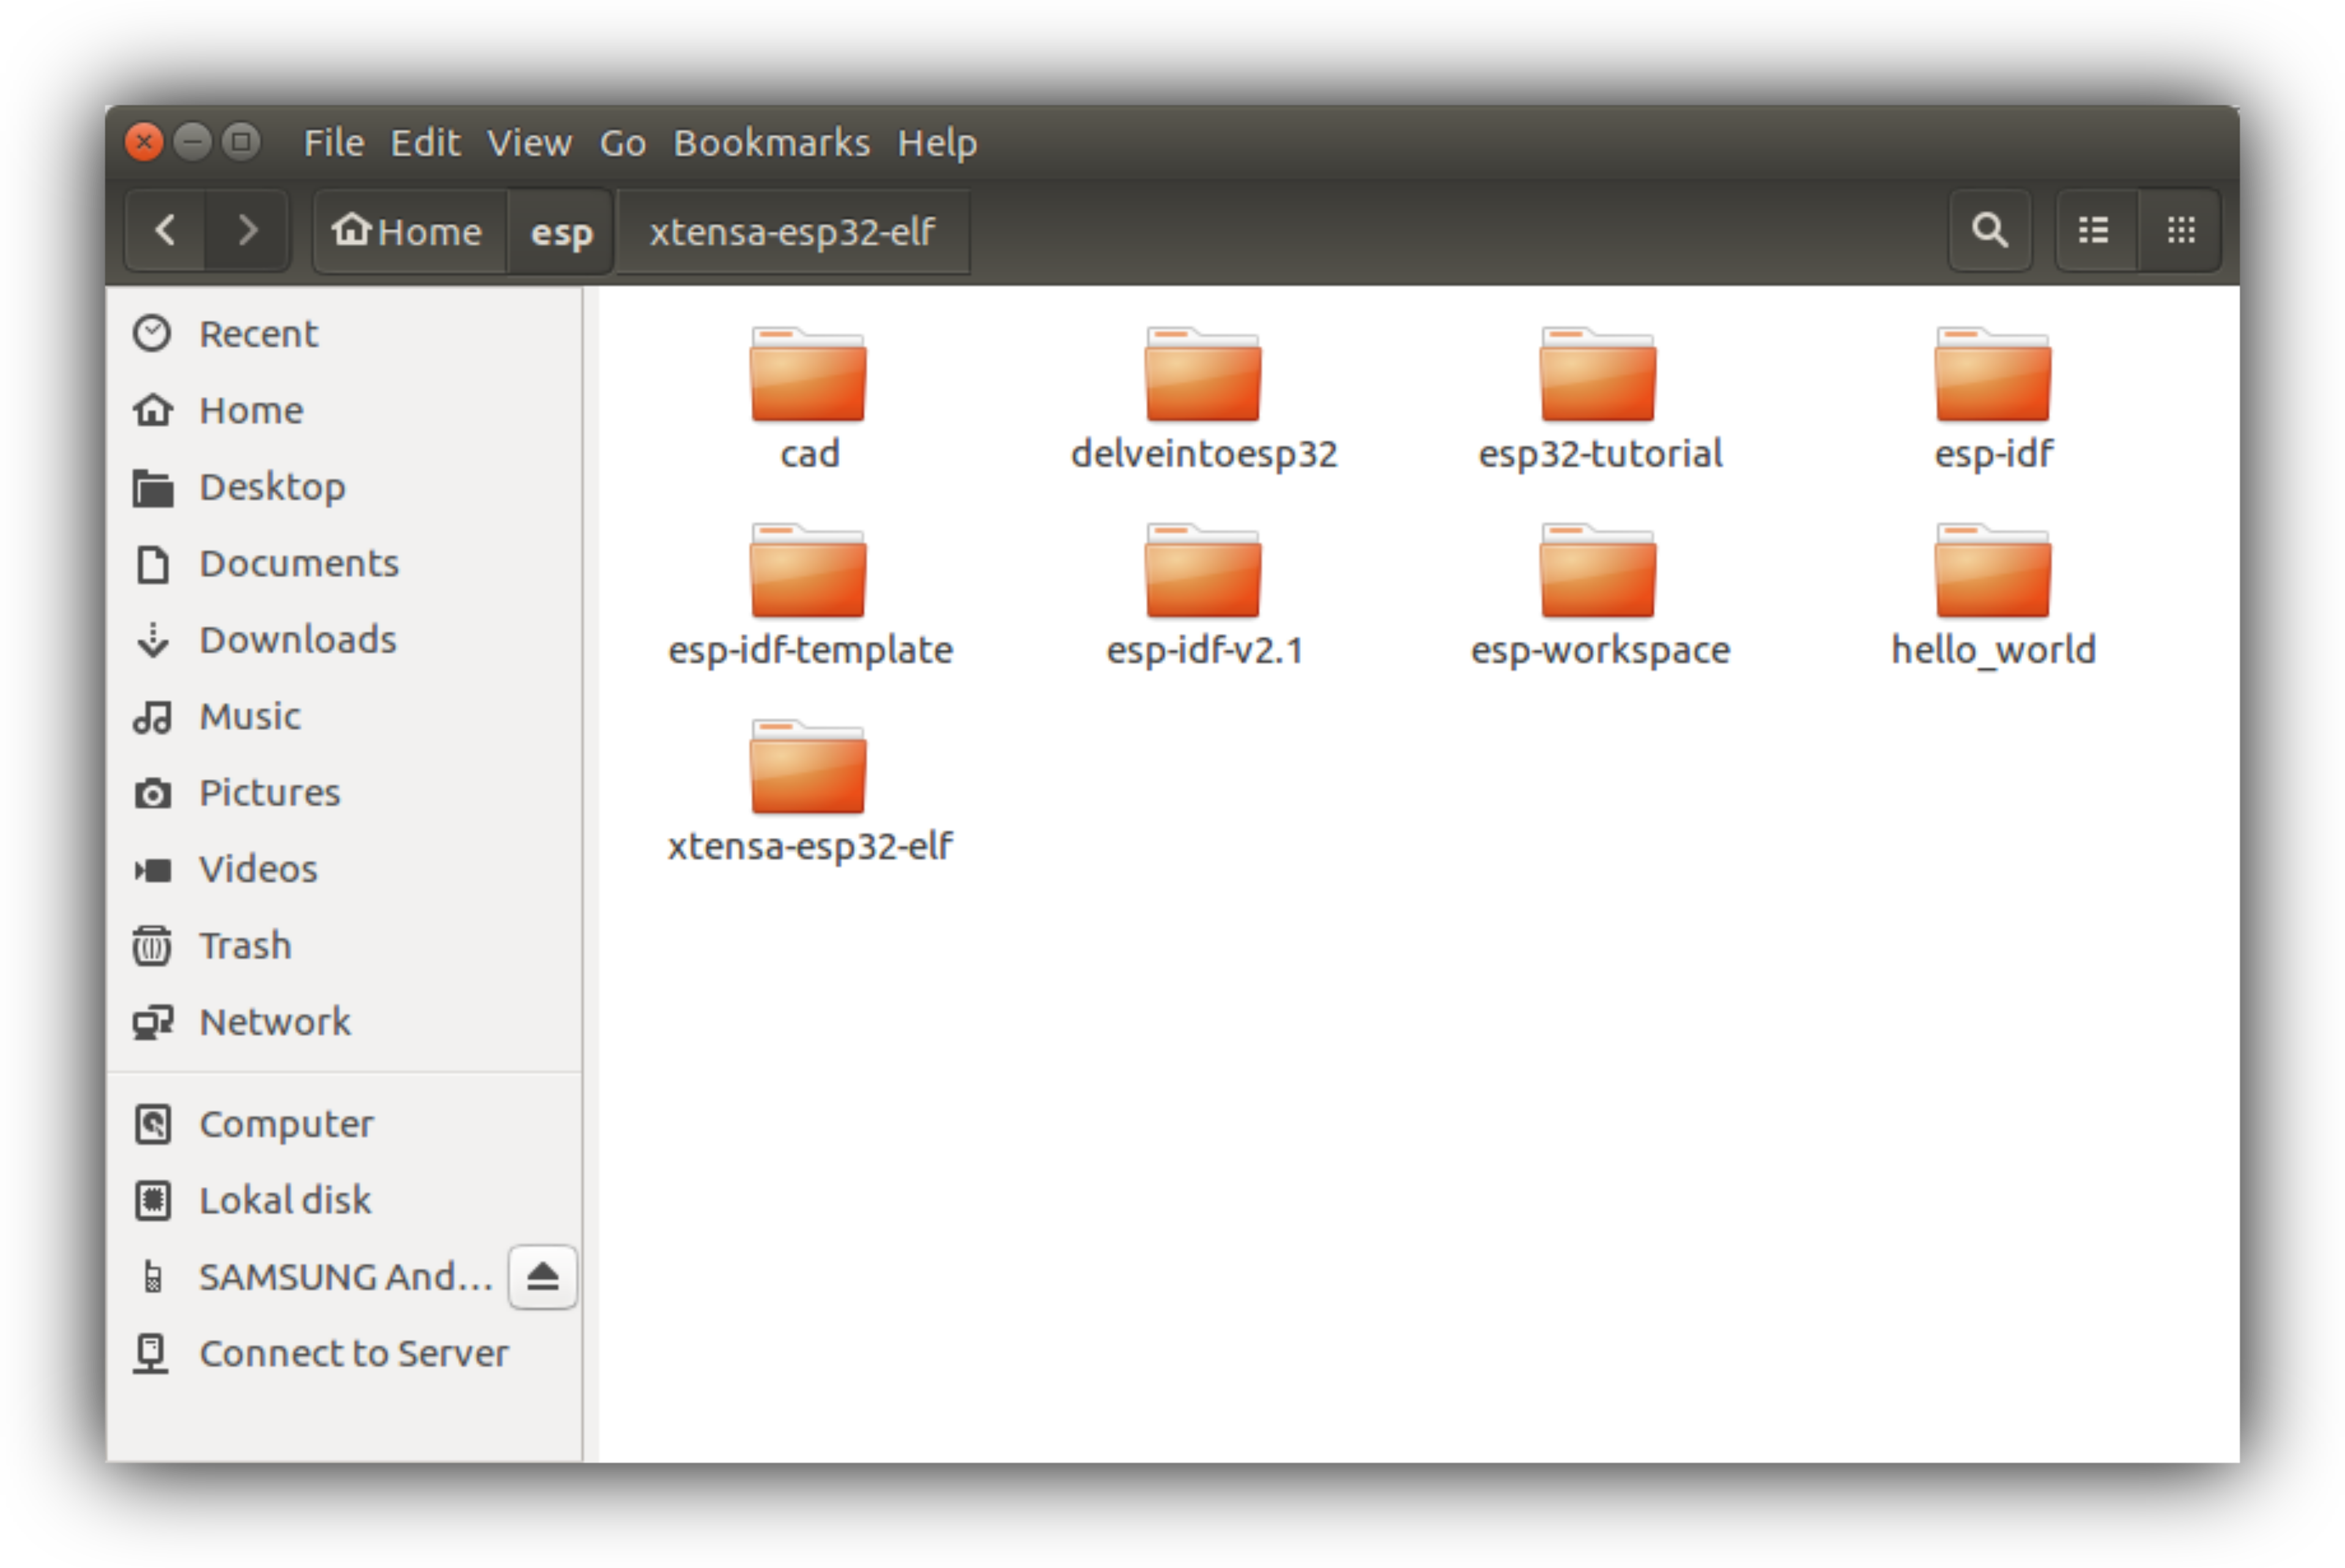
\includegraphics{tool_chain_folder_shadowed.png}
	\caption[ $n$.][6pt]{The folder xtensa-esp32-elf holds the tool chain. Both this folder and the esp-idf folder have been placed in a folder called esp.}
	\label{fig:tool_chain_folder_shadowed}
\end{figure}

\end{document}
